\chapter{Gradientenabstiegsverfahren}
Das Gradientenabstiegsverfahren oder einfach nur Gradientenverfahren
(engl. \textit{gradient decent})
ist ein allgemeiner Optimierungsalgorithmus
um eine Kostenfunktion zu minimieren \parencite[118]{book:hands-on-ml}.
Man stelle sich vor, man befinde sich auf einem Hügel im dichten Nebel
und möchte das Tal erreichen.
Eine gute Strategie wäre es, die Steigung des
Hügels abzuschätzen und sich dort entlangzubewegen,
wo die Senkung am größten ist.
Das Gradientenverfahren führt genau diese Schritte durch,
es misst die Steigung der Kostenfunktion für alle Parameter
und geht für jeden einen kleinen Schritt in die Richtung des Abhangs.
Betrachten wir eine einfache Kostenfunktion
mit nur einem Parameter:
\begin{equation*}
  J(x) = x^2 
\end{equation*}
Das Optimierungsproblem besteht darin, ein $x$ zu finden, mit dem die Funktion minimiert wird.
Die folgende Schritte beschreiben das Vorgehen:
\begin{enumerate}
  \item Wähle einen zufälligen Startpunkt $x$.
  \item Bestimme die Steigung der Funktion in diesem Punkt.
  \item Mache einen Schritt in Richtung des Abhangs und aktualisiere den $x$-Wert.
  \item Wiederhole Schritt zwei bis drei so lange,
        bis sich $x$ nicht mehr oder nur noch sehr wenig ändert.
\end{enumerate}
Um die Steigung zu bestimmen, muss die Ableitung der Kostenfunktion ermittelt werden.
\autoref{eq:one-step-gd-x2} zeigt einen Durchlauf der eben beschriebenen Schritte.
\begin{equation}
  x = x - \alpha \cdot \frac{\mathrm{d}J}{\mathrm{d}x} = x - \alpha \cdot 2x
  \label{eq:one-step-gd-x2}
\end{equation}
Der Parameter $\alpha$ beschreibt die Schrittweite. Diese wird auch das
Lerntempo genannt (engl. \textit{learning rate}).
Das Gradientenverfahren für unsere Beispielsfunktion kann in Python 
einfach umgesetzt werden:
\begin{pythoncode}
def dJ(x):
    return 2*x

def gradient_descent(start, n_epochs=50, learning_rate=0.01):
    x = start
    for _ in range(n_epochs):
        gradient = dJ(x)
        x = x - learning_rate * gradient
    return x
\end{pythoncode}
Die obere Funktion kann erweitert werden, um die Schritte anzuzeigen,
die der Algorithmus durchführt, wie in \autoref{fig:gd} zu sehen ist.
\begin{figure}[h!]
  \centering
  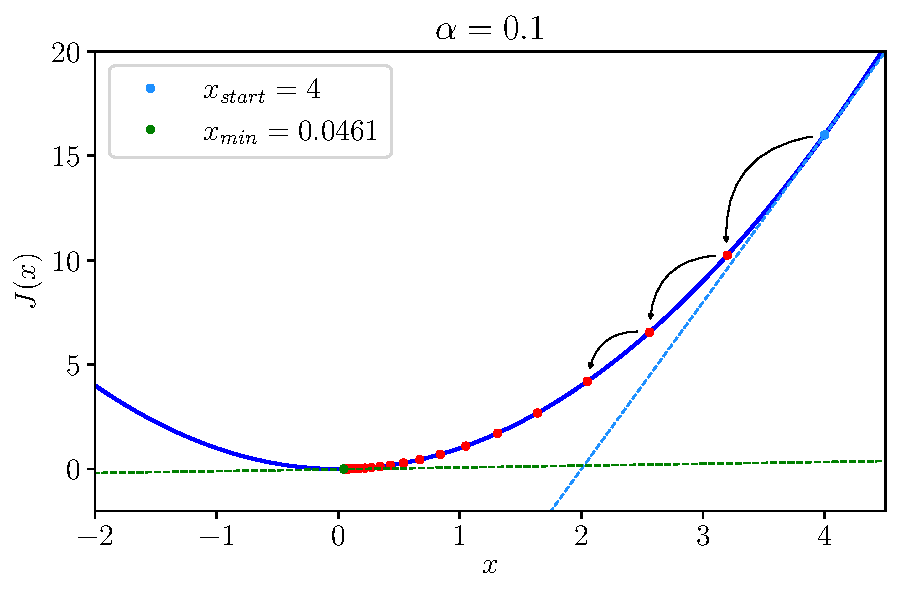
\includegraphics[width=0.7\textwidth]{gradient-decent/gd.pdf}
  \caption{Die ersten 20 Epochen des Gradientenabstiegs und einem Lerntempo von \num{0.1}}
  \label{fig:gd}
\end{figure}

\noindent
Die hellblau gestreifte Linie zeigt die Tangente der Funktion am Startpunkt und
die grün gestreifte Linie am Endpunkt. Nach 20 Epochen hat das Verfahren
den Tiefpunkt der Funktion (bei $x = 0$) fast erreicht.
Wird die Epochenzahl höher eingestellt, kann sich dem Tiefpunkt weiter angenähert werden:
\begin{pyconcode}
>>> x_min = gradient_descent(start=100, n_epochs=1000, learning_rate=0.1)
>>> x_min
1.2302319221611203e-95
\end{pyconcode}
Das Lerntempo ist ein wichtiger Parameter, der ausschlaggebend ist,
wie schnell ein gegebenes Modell trainiert werden kann.
Ist das Lerntempo zu klein, dauert das Training lange,
da der Gradientenabstieg insbesondere an Stellen mit geringer Steigung nur
winzige Schritte durchführt:
\begin{figure}[h!]
  \centering
  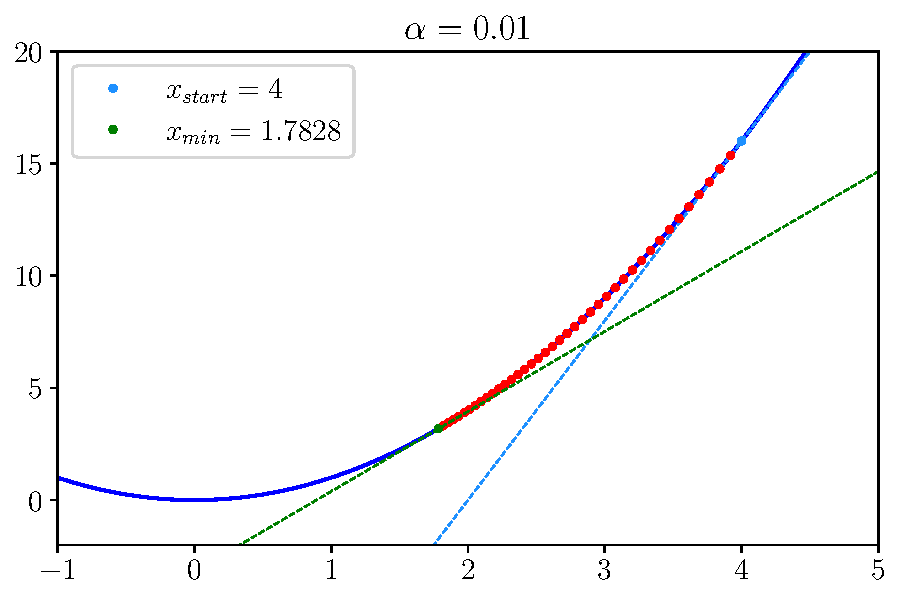
\includegraphics[width=0.7\textwidth]{gradient-decent/gd-low-lr.pdf}
  \caption{Die ersten 40 Epochen des Gradientenabstiegs und einem Lerntempo von \num{0.01}}
  \label{fig:gd-low-lr}
\end{figure}

\noindent
Ist das Lerntempo zu groß, kann es passieren, dass gar keine Lösung gefunden wird
und der $x$-Wert divergiert:
\newpage
\begin{figure}[h!]
  \centering
  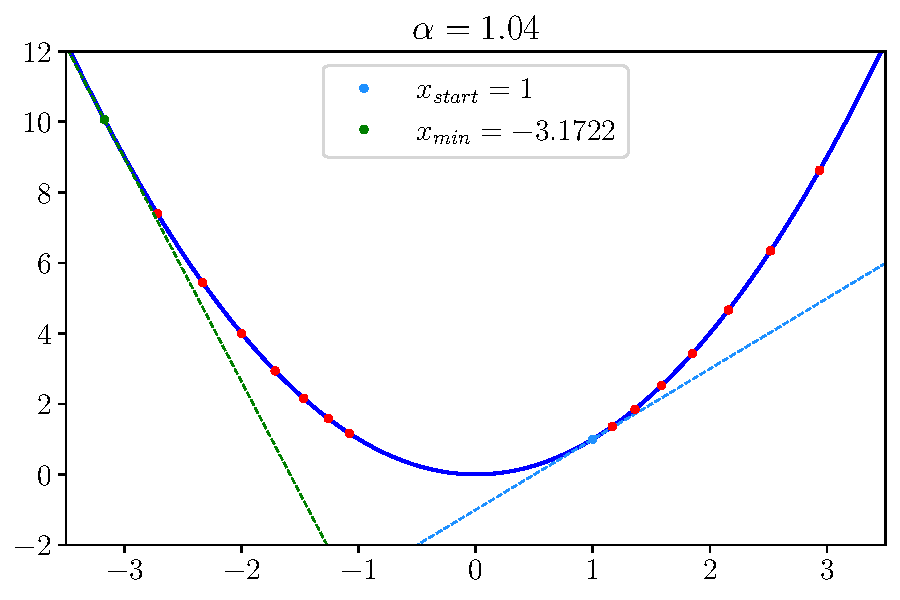
\includegraphics[width=0.7\textwidth]{gradient-decent/gd-high-lr.pdf}
  \caption{Die ersten 15 Epochen des Gradientenabstiegs und zu hohem Lerntempo}
  \label{fig:gd-high-lr}
\end{figure}

\noindent
Ein weiter Vorbehalt des Gradientenverfahrens liegt in der Kostenfunktion.
Nicht alle Kostenfunktionen haben eine so praktische Form wie im bisherigen Beispiel.
Betrachten wir den folgenden Fall:
\begin{figure}[h!]
  \centering
  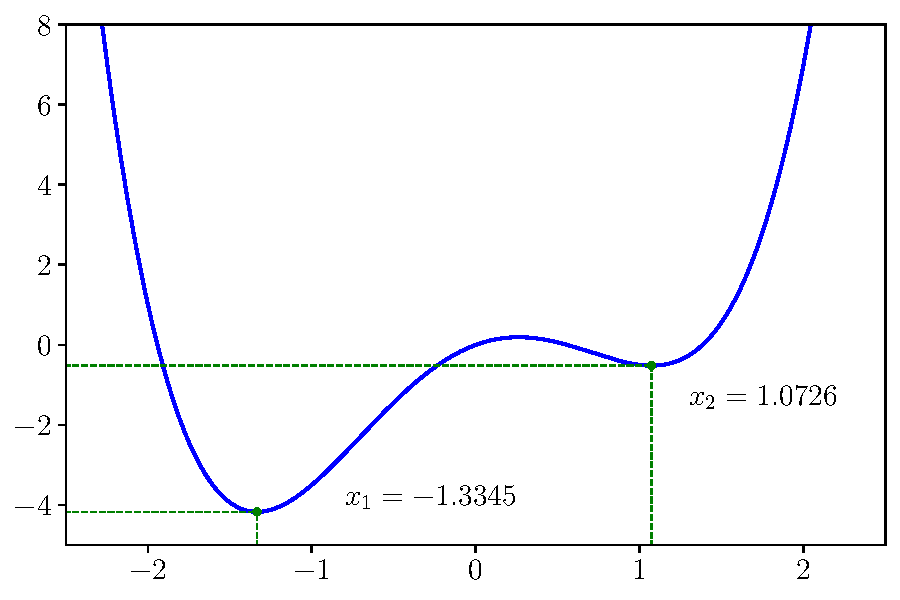
\includegraphics[width=0.7\textwidth]{gradient-decent/mulitple-minima.pdf}
  \caption{Kostenfunktion mit globalem und lokalem Minimum}
  \label{fig:mulitple-minima}
\end{figure}

\noindent
Die Funktion aus \autoref{fig:mulitple-minima} hat sowohl ein globales als auch auch
lokales Minimum. Ein Gradientenabstieg mit Startpunkt auf der rechten Seite würde
zwar einen Tiefpunkt finden, dieser ist jedoch nicht die bestmögliche Lösung des Problems.
\begin{figure}[h!]
  \centering
  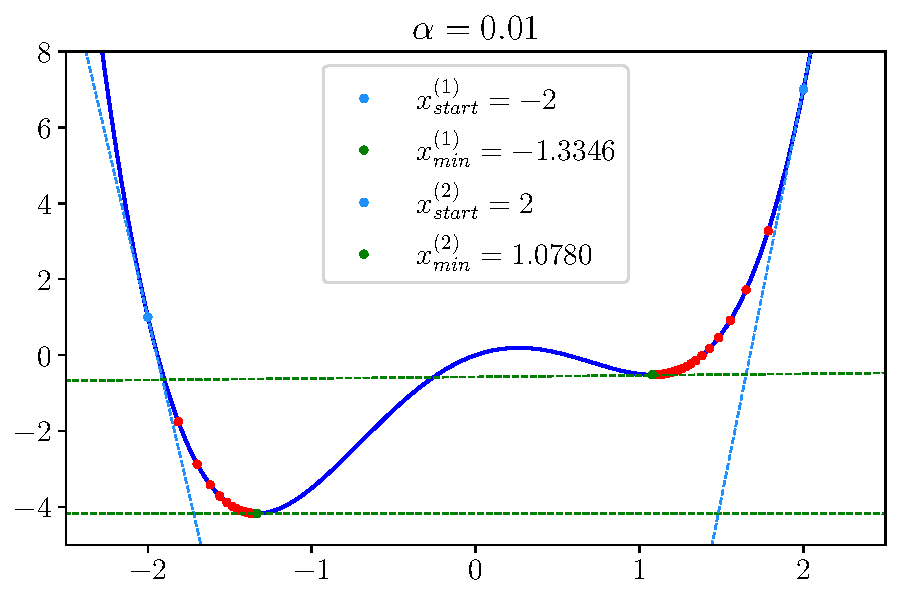
\includegraphics[width=0.7\textwidth]{gradient-decent/gd-mulitple-minima.pdf}
  \caption{Gradientenabstieg hängt im lokalen Minimum}
  \label{fig:gd-mulitple-minima}
\end{figure}

\noindent
Wie in \autoref{fig:gd-mulitple-minima} zu sehen ist, kann
der Gradientenabstieg in lokalen Minima hängen bleiben.
% \begin{listing}[h!]
%   \begin{minted}[escapeinside=||]{text}
%     bis konvergiert:
%       |$w_j = w_j - \alpha \cdot \frac{\partial}{\partial w_j}J(\yhat, y)$|
%   \end{minted}
%   \caption{Das Gradientenverfahren}
% \end{listing}
